\cleardoublepage
\chapter{Cognitive Language Agents for Question Answering}
\label{ch:development}
\label{ch:chapter3}

In this section, we first present the datasets used in our evaluation study, followed by a description of the evaluation framework. This framework supports the development of both the baseline systems and the proposed cognitive language agents. The baseline results are further analyzed in \textit{Analyzing Retrieval Scaling in RAG Systems for Complex QA Benchmarks} \cite{RayoMosquera2025}, a study published as part of this broader research effort.

\section{Methodology}
\subsection{Datasets}

To evaluate our language agents and baselines models, we use three  well-known benchmarks for the MHQA task, \textbf{HotpotQA} \cite{yang2018hotpotqa}, \textbf{2WikiMultiHopQA} \cite{ho-etal-2020-constructing}, and \textbf{MuSiQue} \cite{trivedi2021musique}. Although prior work has shown that \textbf{HotpotQA} does not always require genuine multi-hop reasoning, we include it to support comparison with prior work \cite{trivedi2021musique}.

\noindent All evaluations are performed on the development sets of these datasets, which offer a sufficient number of samples for statistically meaningful results. Following the setup proposed by Bernal et al. \cite{NEURIPS2024_6ddc001d}, we construct a corpus for each dataset by combining the annotated supporting passages with distractor passages. To maintain consistency across evaluations, only answerable questions are retained.

\noindent In addition to the MHQA benchmarks, we evaluate our systems on \textbf{LoCoMo}, a lesser-studied dataset designed for conversational QA \cite{maharana-etal-2024-evaluating}. For this work, we select a smaller subset consisting of 10 conversations. The questions include a mix of multi-hop, temporal, open-domain, and single-hop queries. As with the other datasets, non-answerable questions are excluded. Including LoCoMo allows us to test whether the proposed cognitive agent architectures remain effective in conversational QA scenarios that may be less demanding than standard MHQA tasks.

\noindent Table \ref{tab:dataset_stats} summarizes key statistics of these datasets. MuSiQue and 2WikiMultiHopQA are the most challenging among the selected datasets. Both were explicitly designed to enforce multi-step reasoning and reduce shortcut exploitation by LLMs, making them particularly well-suited for evaluating the reasoning capabilities of our language agents.

\begin{table}[h]
    \centering
    \begin{tabular}[\textwidth]{
        >{\raggedright\arraybackslash}p{2cm}  % Left-aligned and wrapped
        c
        >{\centering\arraybackslash}p{2.5cm}
        >{\centering\arraybackslash}p{2.5cm}
        c
    }
        \toprule
        \textbf{\scriptsize Dataset} &
        \textbf{\scriptsize \# Documents} &
        \textbf{\scriptsize Avg Doc Length (chars)} &
        \textbf{\scriptsize Avg Doc Length (tokens)} &
        \textbf{\scriptsize \# Questions} \\
        \midrule
        LoCoMo\textsuperscript{1} & 5,882 & 207.4 & 54.7 & 1,525 \\
        HotpotQA & 66,609 & 531.9 & 120.2 & 7,405 \\
        2Wiki & 56,680 & 430.8 & 104.1 & 12,576 \\
        MuSiQue & 21,100 & 474.2 & 106.3 & 2,417 \\
        \bottomrule
        \multicolumn{5}{p{14cm}}{\footnotesize \textsuperscript{1} A document corresponds to a single message within a conversation.} \\
    \end{tabular}
    \caption{Dataset statistics.}
    \label{tab:dataset_stats}
\end{table}


\subsection{Evaluation Framework}
\label{evaluation_framework_sec}

We developed an evaluation framework in Python 3.13, publicly available at \href{https://github.com/oyar99/LanguageAgentsQA}{Language Agents QA}, designed to streamline experimentation with the datasets and to facilitate the implementation of both simple RAG baselines and more advanced language agent architectures.

\noindent The framework supports two execution modes: prediction and evaluation. The \textit{orchestrator} is responsible for initiating the appropriate mode, initializing the dataset and agent, and executing the workflow. 

\noindent Each agent implementation must adhere to a common interface that defines two methods: \textit{index} and \textit{reason}. In the \textit{index} method, the agent receives the preprocessed dataset and may construct an index as needed. In the \textit{reason} method, the agent receives a question and must return an object containing the final answer, the list of documents consulted during reasoning, and additional metadata such as token usage. 

\begin{figure}[h]
    \centering
    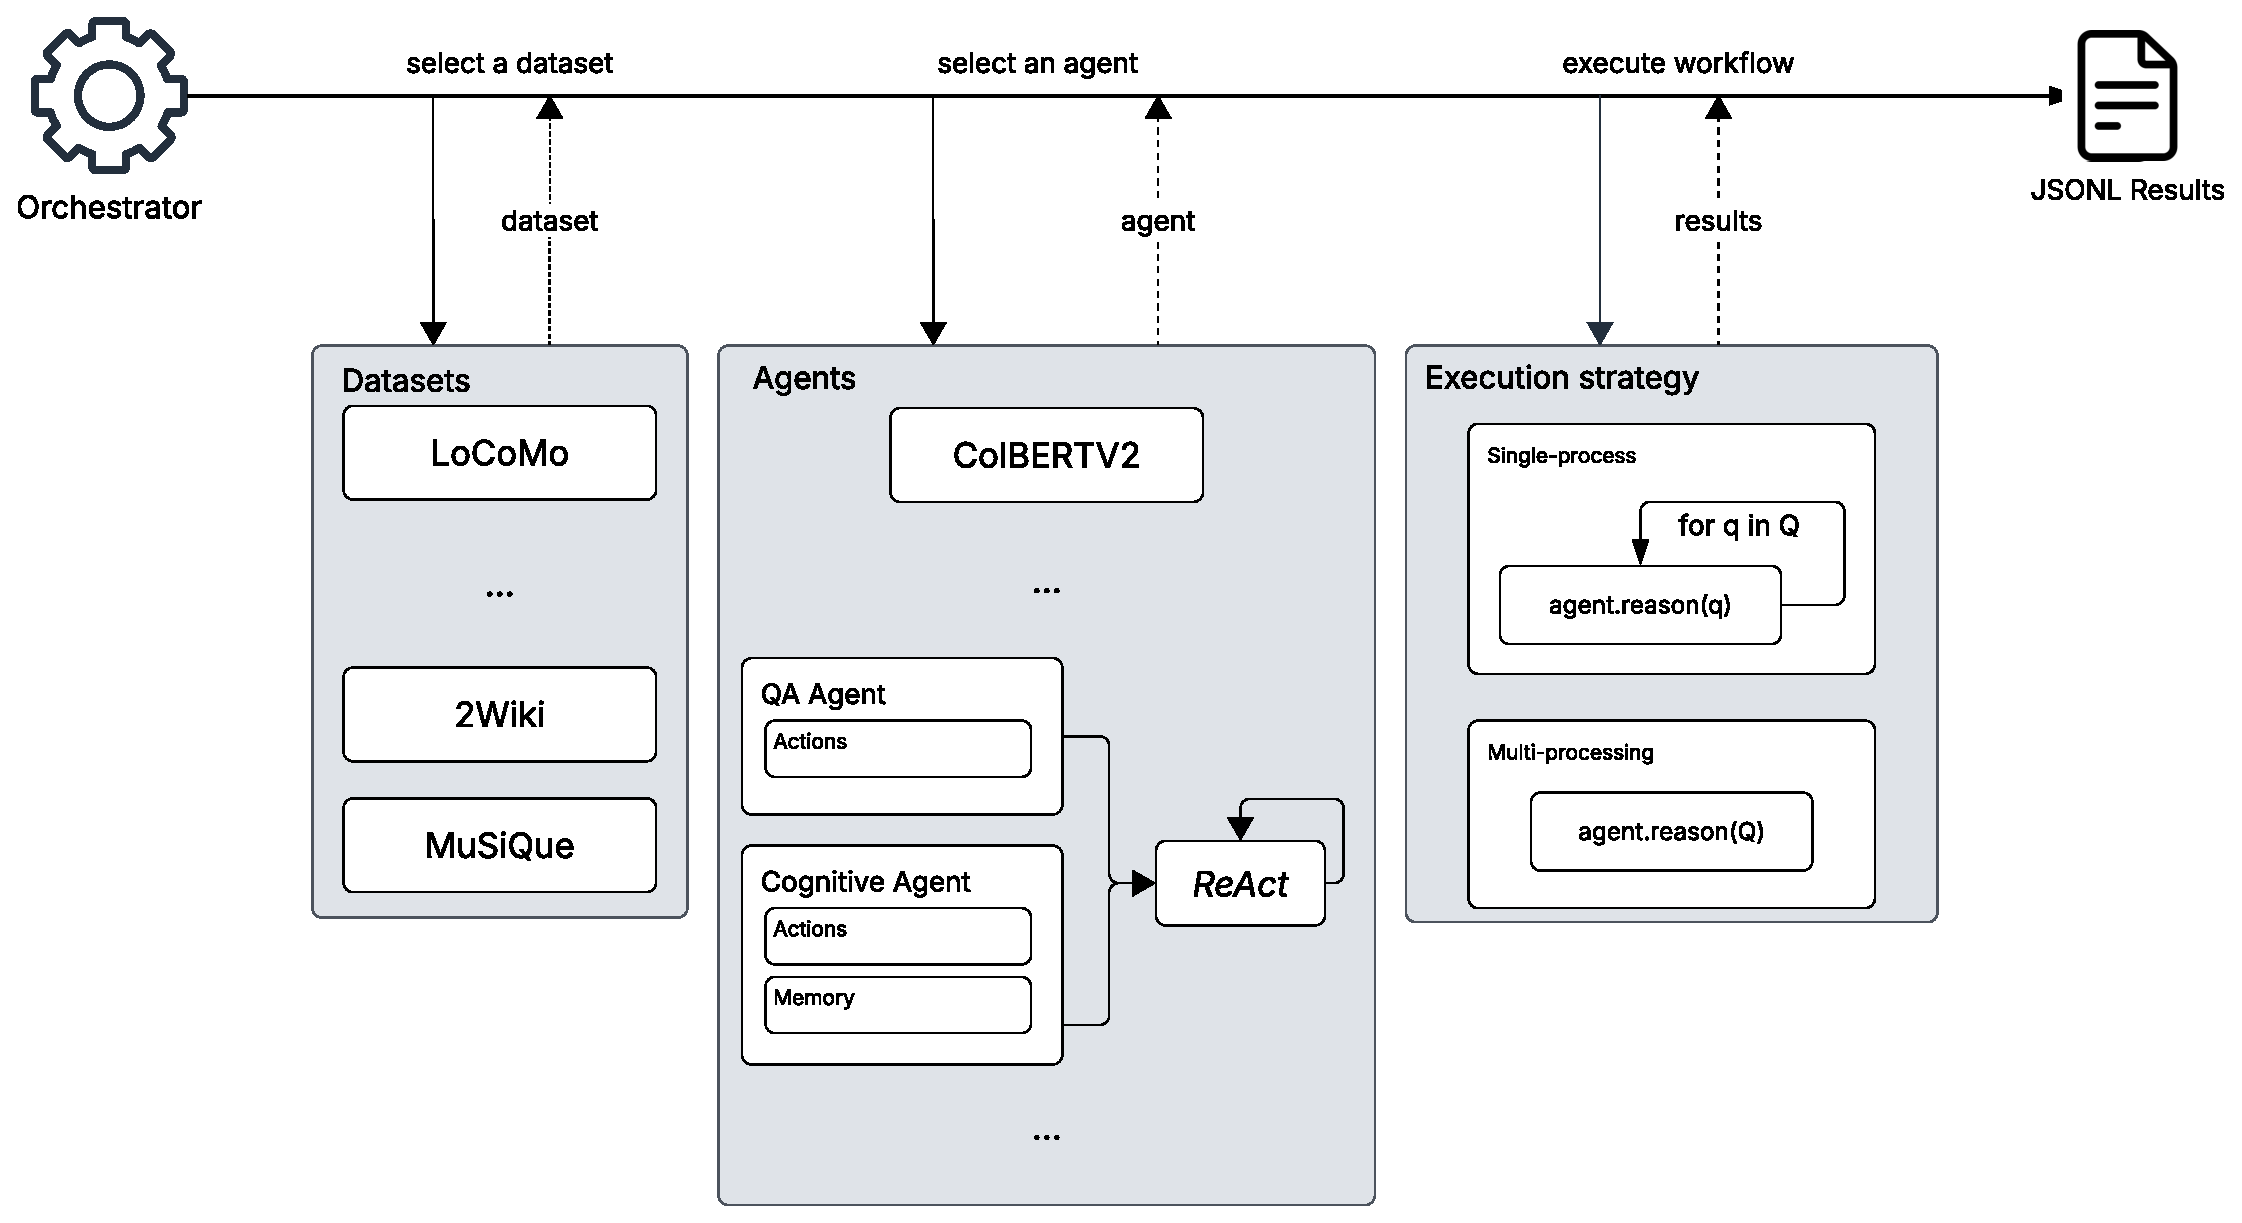
\includegraphics[width=1\textwidth]{images/eval-framework.eps}
    \caption{Evaluation framework architecture in prediction mode. The orchestrator (i) loads and initializes the dataset, (ii) configures the selected agent, and (iii) executes the question-answering workflow with the appropriate execution strategy.}
    \label{fig:eval_frame}
\end{figure}

\noindent The framework also provides a base implementation for more sophisticated agents. In particular, it includes an abstract ReAct agent that must be initialized with a set of actions. These actions, representing the agent's procedural memory, are Python functions paired with concise natural language descriptions. The base agent implements the ReAct reasoning loop following a structured well-defined JSON format. This implementation is designed for extensibility and can serve as the underlying reasoning engine for other agents. Importantly, the architecture is flexible enough to also implement baseline methods described in Section \ref{baselines_sec}, even when those methods are not strictly agent-based. An overview of the framework is provided in Figure \ref{fig:eval_frame}.

\noindent In evaluation mode, the script accepts a path to a JSONL file containing results and reports both retrieval and QA metrics, including recall, precision, $F_1$, recall@k, $EM$, $R_1$, $R_2$, and $L_1$.  

\noindent Furthermore, the framework supports multiprocessing, enabling independent processing of questions. In our experiments, we usually leverage  up to 40 CPUs, substantially reducing runtime.

\noindent Finally, the framework integrates with vLLM, an inference and serving engine for LLMs. Any generative model available in vLLM can be used through the same interface as OpenAI's chat completions endpoint \cite{kwon2023efficient}.

\subsection{Baselines}
\label{baselines_sec}

We evaluated a range of retrieval systems, including both traditional lexical and semantic retrievers, as well as more advanced methods.

\noindent First, we used a BM25 ranking function with hyperparameters $b = 0.75$ and $k_1 = 0.5$. These values were selected experimentally, considering that passages across all four datasets are relatively short \cite{10.1145/2682862.2682863}. Both  documents and queries were processed through a standard normalization pipeline that includes unigram and bigram generation, stopword removal, Snowball stemming, and other text normalization techniques.

\noindent Second, we evaluated a semantic retriever based on the msmarco-bert-base-dot-v5 model, which encodes text into a 768-dimensional embedding space. This model, trained on question answer pairs from the MS Marco dataset, has demonstrated strong performance on a range of natural language tasks including QA \cite{reimers-2019-sentence-bert}.

\noindent Third, we included ColBERTv2, a semantic retriever that leverages contextual late interaction. Unlike single-vector dense retrievers, ColBERTv2 compares queries and documents at the token level, allowing for finer-grained relevance retrieval \cite{santhanam-etal-2022-colbertv2}.

\noindent To explore retrieval methods that leverage structured knowledge, we evaluated HippoRAG, a recent architecture inspired by neurobiological systems. HippoRAG constructs a knowledge graph by extracting triples from the corpus using an LLM. In our experiments, we used both QWen2.5-14B-Instruct and GPT-4o-mini \cite{qwen2}. HippoRAG also uses a dense embedding model during both indexing and QA \cite{NEURIPS2024_6ddc001d}, in our case Contriever \cite{lei-etal-2023-unsupervised}. This structured representation enables competitive performance, particularly on more challenging datasets such as MuSiQue.

\noindent To construct a strong baseline for these retrievers, we implemented several standard RAG systems, with carefully designed QA prompt templates to maximize question answering scores. (See Appendix \ref{ch:appendices}). For each system, we varied the number of retrieved passages $k$, from $5$ to $100$, to assess the impact of effective context length on performance. We also tested a FULL-CONTEXT variant in which all documents are provided to the model, ensuring that relevant ground-truth passages are always included, even if truncation is needed to fit within the model's context window. Due to computational constraints, questions in the FULL-CONTEXT setting are processed in batches of size 8, and the model is required to return structured outputs to locate the answer to each question deterministically. While this multitask scenario is not directly comparable with the RAG baselines, it offers useful insight into how model performance scales as more context is used.

\noindent The baselines used GPT-4o-mini (2024-07-18) with a context window of $128k$ tokens. We used the OpenAI API using version 2024-12-01-preview, utilizing both the chat completions and batch processing endpoints for cost efficiency.

\noindent We also report results obtained with QWen2.5-14B-Instruct, which supports a $32K$ token context window \cite{qwen2}. This model was executed using vLLM with 16-bit floating precision on two NVIDIA A40 GPUs, each with 46GB of VRAM \cite{kwon2023efficient}.

\noindent For a few scenarios, we additionally evaluated o3-mini (2025-01-31), which provides a $200k$ token context window. For this model, we selected the medium reasoning effort configuration.

\noindent All models were run with temperature set to $0$ to ensure outputs are as deterministic as possible, and frequency and presence penalties were also set to $0$. The maximum number of completion tokens was set to $500$, which we found sufficient, as most answers are brief. Additionally, we designated the newline character (\textbackslash n) as a stop token, since many models, particularly smaller ones, struggled to adhere to the output formatting instructions and often appended additional commentary.

\subsection{Cognitive Language Agents}
\label{agents_sec}

Building on the evaluation framework, we design several language agent architectures aimed at improving QA performance. All agents are grounded in the \textbf{ReAct} framework, which interleaves reasoning and action. Actions typically correspond to search functions, and agents may also decompose complex questions into sub-questions to facilitate multi-step reasoning. The base prompt used to guide these agents is shown in Figure \ref{fig:agent_base_prompt}, and individual variants adapt it with specific tools, tool descriptions, or illustrative examples.

\subsubsection{QA Agent}

\noindent The simplest variant defines a single action: retrieving relevant passages using ColBERTv2 with a fixed retrieval depth of $k = 5$. Once sufficient context is gathered, the agent produces an answer. This agent uses GPT-4o-mini, and includes two examples as context. The architecture is shown in Figure \ref{fig:qa_agent}.

\begin{figure}[h]
    \centering
    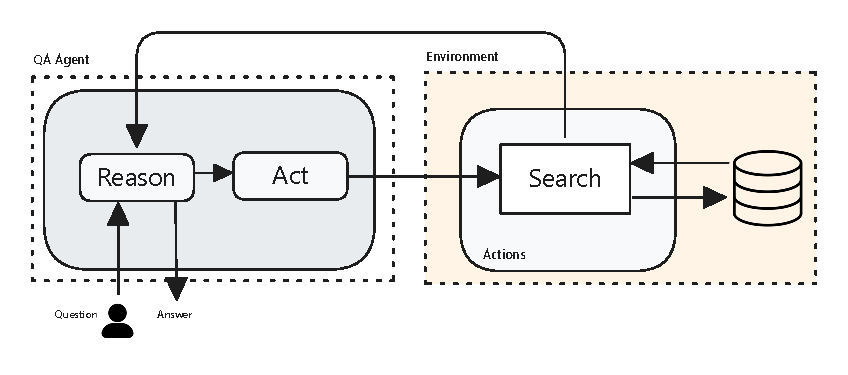
\includegraphics[width=1\textwidth]{images/qa_agent}
    \caption{QA Agent architecture using ReAct.}
    \label{fig:qa_agent}
\end{figure}

\subsubsection{QA Agent with Re-ranking}

\noindent This agent extends the QA agent by introducing an LLM-based second-stage retriever that re-ranks the initial retrieval set. The retriever prioritizes higher-quality evidence and discards distractors before reasoning proceeds, thereby improving retrieval precision. Both the second-stage retriever and the agent are tested with GPT-4o-mini. The agent is shown in Figure \ref{fig:qa_reranking_agent}.

\begin{figure}[h]
    \centering
    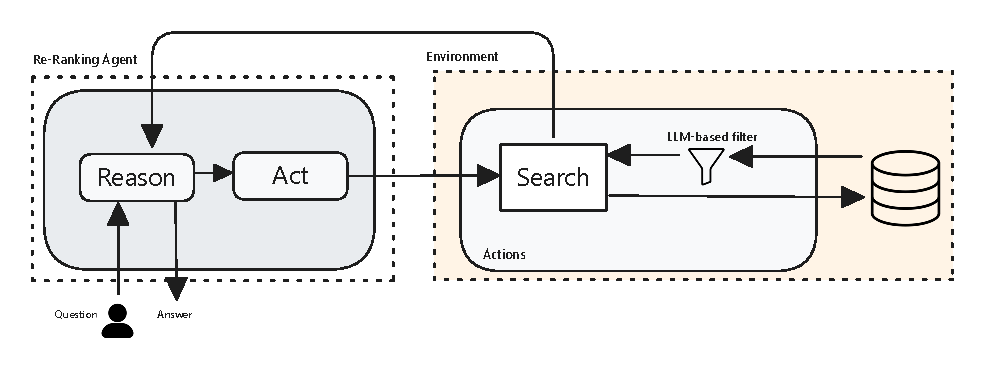
\includegraphics[width=1\textwidth]{images/reranking_agent.eps}
    \caption{QA Agent with re-ranking support.}
    \label{fig:qa_reranking_agent}
\end{figure}

\subsubsection{QA Agent with Pagination}

\noindent This variant augments the search tool with a \textit{page} parameter, allowing the agent to retrieve additional results beyond the initial retrieval set. For example, calling \textit{search('northwestern Somalia', 2)} returns passages ranked from position 6 to 10. This mechanism enables exploration of a broader retrieval space when necessary.

\subsubsection{Cognitive Agent}

\noindent We propose a cognitive language agent that incorporates episodic memory to store information about the questions it has answered during its lifetime. Unlike the previously described agents, this agent lifetime extends beyond a single QA session. The memory schema is shown in Figure \ref{fig:mem-schema}.

\begin{figure}[!htbp]
    \centering
    \lstinputlisting{./chapter3/cognitive_agent_memory_schema.txt}
    \caption{Long-term memory schema.}
    \label{fig:mem-schema}
\end{figure}

\begin{figure}[!htbp]
    \centering
    \lstinputlisting{./chapter3/prompt_base_agent.txt}
    \caption{ReAct agent prompt.}
    \label{fig:agent_base_prompt}
\end{figure}

\noindent Like the previous agents, it follows a ReAct loop, but with one key distinction, after generating an answer, the agent evaluates it against the ground truth, simulating a human-in-the-loop process. If the answer is correct, the reasoning trace is stored directly in memory. Otherwise, the agent reflects on the error, reconstructs a reasoning trace that would have led to the correct answer, and stores that instead.

\noindent An example of this reasoning trace format is provided in Figure \ref{fig:reasoning_chain}. When the agent is presented with a new question, it searches for up to $4$ semantically similar questions it has processed before using all-MiniLM-L6-v2, an embedding model that maps text to a 384-dimensional space \cite{reimers-2019-sentence-bert}. It then uses these questions as context for the current question. Over time, this architecture allows the agent to learn from experience and improve its performance, particularly on questions similar to those it has encountered before. Figure \ref{fig:cognitive_agent} illustrates the overall workflow.

\begin{figure}[h]
    \centering
    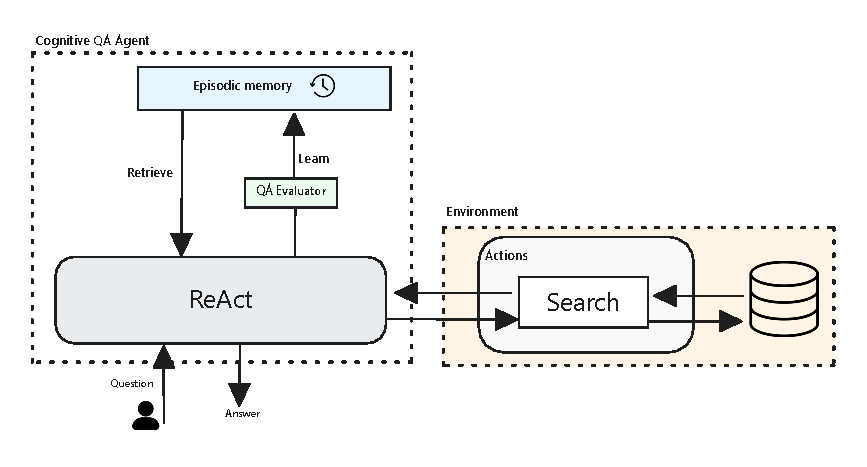
\includegraphics[width=1\textwidth]{images/cognitive_agent.eps}
    \caption{Cognitive Agent architecture.}
    \label{fig:cognitive_agent}
\end{figure}

\begin{figure}[h]
    \centering
    \lstinputlisting{./chapter3/reasoning_chain_sample.txt}
    \caption{Reasoning traces for question \textit{Because Marc Shiller was born in Beunos Aires in 1957, but is a resident of the United States, what ethnic group does he belong to?}}
    \label{fig:reasoning_chain}
\end{figure}

\subsubsection{Cognitive Agent - Search tools}

\noindent We propose a hybrid retrieval cognitive agent that selects among multiple retrieval strategies, lexical, semantic, or graph-based, depending on the characteristics of the input query. As opposed to systems such AriGraph and HippoRAG, which rely on a single search mechanism \cite{anokhin2024arigraphlearningknowledgegraph}\cite{NEURIPS2024_6ddc001d}, our agent flexibly integrates different retrieval strategies, and learns progressively how to best leverage them by building on top of the Cognitive Agent architecture.

\subsubsection{Multi-Agent Reflection}

\noindent We design a multi-agent architecture where one agent, responsible for answering questions, interleaves reasoning, action, and feedback from another agent that verifies whether the reasoning process is correct. This interleaved reflection allows the reasoning agent to adjust its trajectory in real time based on feedback. We experiment with different models for each agent to obtain varying results.

\noindent Finally, these agent are compared against baseline approaches, providing an analysis of their effectiveness, including discussion on system complexity, performance trade-offs, and resource efficiency.